\documentclass{article}

%% PAQUETES

% Paquetes generales
\usepackage[margin=2cm, paperwidth=210mm, paperheight=297mm]{geometry}
\usepackage[spanish]{babel}
\usepackage[utf8]{inputenc}
\usepackage{gensymb}

% Paquetes para estilos
\usepackage{textcomp}
\usepackage{setspace}
\usepackage{colortbl}
\usepackage{color}
\usepackage{color}
\usepackage{upquote}
\usepackage{xcolor}
\usepackage{listings}
\usepackage{caption}
\usepackage[T1]{fontenc}
\usepackage[scaled]{beramono}

% Paquetes extras
\usepackage{amssymb}
\usepackage{float}
\usepackage{graphicx}
\usepackage{url}
\usepackage[toc,page]{appendix}
\usepackage{mips}

% Paquete Matematica
\usepackage{mathtools}


%% Fin PAQUETES


% Definición de preferencias para la impresión de código fuente.
%% Colores
\definecolor{gray99}{gray}{.99}
\definecolor{gray95}{gray}{.95}
\definecolor{gray75}{gray}{.75}
\definecolor{gray50}{gray}{.50}
\definecolor{keywords_blue}{rgb}{0.13,0.13,1}
\definecolor{comments_green}{rgb}{0,0.5,0}
\definecolor{strings_red}{rgb}{0.9,0,0}

%% Caja de código
\DeclareCaptionFont{white}{\color{white}}
\DeclareCaptionFont{style_labelfont}{\color{black}\textbf}
\DeclareCaptionFont{style_textfont}{\it\color{black}}
\DeclareCaptionFormat{listing}{\colorbox{gray95}{\parbox{16.78cm}{#1#2#3}}}
\captionsetup[lstlisting]{format=listing,labelfont=style_labelfont,textfont=style_textfont}

\lstset{
	aboveskip = {1.5\baselineskip},
	backgroundcolor = \color{gray99},
	basicstyle = \ttfamily\footnotesize,
	breakatwhitespace = true,   
	breaklines = true,
	captionpos = t,
	columns = fixed,
	commentstyle = \color{comments_green},
	escapeinside = {\%*}{*)}, 
	extendedchars = true,
	frame = lines,
	keywordstyle = \color{keywords_blue}\bfseries,
	language = C,                       
	numbers = left,
	numbersep = 5pt,
	numberstyle = \tiny\ttfamily\color{gray50},
	prebreak = \raisebox{0ex}[0ex][0ex]{\ensuremath{\hookleftarrow}},
	rulecolor = \color{gray75},
	showspaces = false,
	showstringspaces = false, 
	showtabs = false,
	stepnumber = 1,
	stringstyle = \color{strings_red},                                    
	tabsize = 2,
	title = \null, % Default value: title=\lstname
	upquote = true,                  
}

%% FIGURAS
\captionsetup[figure]{labelfont=bf,textfont=it}
%% TABLAS
\captionsetup[table]{labelfont=bf,textfont=it}

% COMANDOS

%% Titulo de las cajas de código
\renewcommand{\lstlistingname}{Código}
%% Titulo de las figuras
\renewcommand{\figurename}{Figura}
%% Titulo de las tablas
\renewcommand{\tablename}{Tabla}
%% Referencia a los códigos
\newcommand{\refcode}[1]{\textit{Código \ref{#1}}}
%% Referencia a las imagenes
\newcommand{\refimage}[1]{\textit{Imagen \ref{#1}}}

%% APENDICES
\addto\captionsspanish{
	\renewcommand\seename{Apéndices}
	\renewcommand\appendixname{Apéndices}
	\renewcommand\appendixpagename{Apéndices}
}


\begin{document}
\pagenumbering{roman}
\setcounter{page}{5}

% TÍTULO, AUTORES Y FECHA
\begin{titlepage}
	\vspace*{\fill}
	\begin{center}
		\huge{Trabajo Pŕactico N°1} \\
		\medskip
		\Huge \textit{``Conjunto de instrucciones MIPS''} \\
		
		\bigskip\bigskip\bigskip\bigskip\bigskip

		\Large Belén Beltran, Padrón Nro. 91.718 \\
		\large \textit{belubeltran@gmail.com} \\ \medskip
		\Large Pablo Ariel Rodriguez, Padrón Nro. 93.970 \\
		\large \textit{prodriguez@fi.uba.ar} \\ \medskip
		\Large Federico Martín Rossi, Padrón Nro. 92.086 \\
		\large \textit{federicomrossi@gmail.com} \\

		\bigskip\bigskip\bigskip\bigskip\bigskip\bigskip\bigskip

		\large 2do. Cuatrimestre 2013 \\ \smallskip
		\large 66.20 Organización de Computadoras \\ \smallskip
		\large Facultad de Ingeniería, Universidad de Buenos Aires \\ \smallskip

		\date{}
	\end{center}
	\vspace*{\fill}
\end{titlepage}

\newpage
\newpage \textit{}
\newpage



% ÍNDICE
\tableofcontents
\newpage \textit{}
\newpage
\pagenumbering{arabic}




% Introducción
\section{Introducción}
	
	En el presente trabajo se tiene como objetivo la comparación entre dos algoritmos de ordenamiento: el \textit{Bubblesort}\cite{BS} y el \textit{Heapsort}\cite{HS}.
	Para realizar dicha comparación entre ambos se realizó la implementación en lenguaje C de cada uno de estos. A su vez, para comparar el rendimiento entre código de alto nivel y de código nativo, se desarrollo la implementación del Heapsort en assembly MIPS, con el fin de poder comparar los tiempos de ejecución de ambos programas y realizar así un estudio de las mejoras que se producen.
	\par
	La totalidad del trabajo se ha realizado en una plataforma \textit{NetBSD/MIPS-32} mediante el \textit{GXEmul} \cite{GXEMUL}.
	\par
	Todos los archivos y códigos fuente aquí mencionados, así como también el presente informe, pueden ser descargados como un archivo comprimido ZIP del repositorio del grupo\footnote{URI del Repositorio: \url{https://github.com/federicomrossi/6620-trabajos-practicos-2C2013/tree/master/tp1}}.
\bigskip




% Compilación
\section{Compilación}
	
	
	La herramienta para compilar tanto el código asembly como C será el \textit{GCC} \cite{GCC}. 
	\par
	Para automatizar las tareas de compilación se hace uso de la herramienta \textit{GNU Make}. Los Makefiles utilizados para la compilación se incluyen junto al resto de los archivos fuentes del presente trabajo \footnote{Los archivos se encuentran separados según la implemetación a la que pertenecen, por lo que habrán dos Makefiles distintos, uno para la implementación en lenguaje C y otro para la implementación en assembly}.
\bigskip



% Utilización
\section{Utilización}
	
	En los siguientes apartados se especifica la forma en la que deben ser ejecutados los programas implementados tanto en C como en assembly MIPS.
\medskip


% Utilización - Implementación en C
\subsection{Implementación en C}

	El resultado de compilación utilizando el comando \textit{make} será un archivo ejecutable de nombre \textit{tp1}, que podrá ser invocado con los siguientes parámetros:
	\medskip

	\begin{itemize}

		\itemsep=2pt \topsep=0pt \partopsep=0pt \parskip=0pt \parsep=0pt
			\item \textit{-h}:  Imprime ayuda para la utilización del programa;
			\item \textit{-V}:  Imprimer la versión actual del programa;
			\item \textit{-b [ARGS]}:  El programa recibe nombres de archivos de texto o strings ingresados por \textit{stdin}, ordenandolos utilizando el algoritmo Bubblersort. Para utilizar \textit{stdin} deberá ingresarse el caracter '-' y luego introducir las palabras;
			\item \textit{-p [ARGS]}:  El programa recibe nombres de archivos de texto o strings ingresados por \textit{stdin}, ordenandolos utilizando el algoritmo Heapsort. Para utilizar \textit{stdin} deberá ingresarse el caracter '-' y luego introducir las palabras.

	\end{itemize}	
	\medskip



\subsection{Implementación en Assembly}

	El resultado de compilación utilizando el comando \textit{make} será un archivo ejecutable de nombre \textit{tp1}, el cual aceptará un archivo de texto como argumento y lo ordenará con el algoritmo Heapsort.
\bigskip\bigskip




% Implementación
\section{Implementación}
	
	En lo que sigue de la sección, se presentarán los códigos fuente de la implementación del algoritmo. Aquellos lectores interesados en la implementación completa del programa, pueden dirigirse al apéndice ubicado al final del presente informe.
\bigskip



% Implementación en C
\subsection{Implementación en C}

	La implementación del programa fue divida en los siguientes módulos:
	\medskip

\begin{itemize}

\itemsep=2pt \topsep=0pt \partopsep=0pt \parskip=0pt \parsep=0pt
	\item \textbf{tp1}: Programa principal responsable de interpretar los comandos pasados por la terminal de modo que realice las tareas solicitadas por el usuario. Su principal función es encadenar el funcionamiento de los otros módulos y mostrar por pantalla el resultado obtenido;
	\item \textbf{bubblesort}: Módulo encargado de implementar el algoritmo de ordenamiento Bubblesort. Recibe como parámetros un arreglo de palabras desordenado y el tamaño del mismo. Como resultado devuelve dicho arreglo ordenado.
	\item \textbf{heapsort}: Módulo encargado de implementar el algoritmo de ordenamiento Heapsort. Recibe como parámetros un arreglo de palabras desordenado y el tamaño del mismo. Como resultado devuelve dicho arreglo ordenado.

\end{itemize}	
\medskip


% Algoritmo Bubblesort 
\subsubsection{Algoritmo \textit{Bubblesort}}

	En el \refcode{codeBSh} se muestra el header de la librería, donde se declara la función \textit{bubblesort}, mientras que en el \refcode{codeBSc} se muestra la definición de la librería.

% Código
\lstset{ language = C } % Cambiamos el lenguaje para que parsee en C
\lstinputlisting[label=codeBSh,caption=``bubblesort.h'']{../codigo/c/bubblesort.h} 
\bigskip


% Código
\lstset{ language = C } % Cambiamos el lenguaje para que parsee en C
\lstinputlisting[label=codeBSc,caption=``bubblesort.c'']{../codigo/c/bubblesort.c} 
\bigskip




% Algoritmo Heapsort
\subsubsection{Algoritmo \textit{Heapsort}}

	En el \refcode{codeHSh} se muestra el header de la librería, donde se declara la función \textit{heapsort}, mientras que en el \refcode{codeHSc} se muestra la definición de la librería.

% Código
\lstset{ language = C } % Cambiamos el lenguaje para que parsee en C
\lstinputlisting[label=codeHSh,caption=``heapsort.h'']{../codigo/c/heapsort.h} 
\bigskip


% Código
\lstset{ language = C } % Cambiamos el lenguaje para que parsee en C
\lstinputlisting[label=codeHSc,caption=``heapsort.c'']{../codigo/c/heapsort.c} 
\bigskip\bigskip
\newpage


% Implementación en Assembly
\subsection{Implementación en Assembly}

	La implementación del programa fue divida en los siguientes módulos:
	\medskip

\begin{itemize}

\itemsep=2pt \topsep=0pt \partopsep=0pt \parskip=0pt \parsep=0pt
	\item \textbf{tp1}: Solamente recibe un texto como argumento por linea de comandos y lo imprime ordenandolo mediante heapsort. Esta implementado en lenguaje C;
	\item \textbf{strcmpi}: Función implementada en assembly MIPS que se encarga de realizar la comparación de strings sin ser sensible a mayúsculas;
	\item \textbf{heap}: Función implementada en assembly MIPS que se encarga de armar la estructura heap que es necesaria en cada paso del heapsort;
	\item \textbf{heapsort}: Implementación en assembly MIPS del algoritmo de ordenamiento Heapsort.

\end{itemize}	
\medskip




% Algoritmo Heapsort
\subsubsection{Algoritmo \textit{Heapsort}}

	En el \refcode{codeHSaMED} se muestra la implementación en assembly del algoritmo Heapsort.

% Código
\lstset{ language = [mips]Assembler} % Cambiamos el lenguaje para que parsee en MIPS
\lstinputlisting[label=codeHSaMED,caption=``heapsort.S'']{../codigo/assembly/heapsort.S} 
\bigskip\bigskip\medskip



% Debugging
\section{Debugging}
	
	Para analizar el correcto funcionamiento del programa se crearon casos de prueba pertinentes, considerando combinaciones diferentes en el ingreso de parámetros al programa principal, como también tomando en cuenta las diferentes salidas obtenidas a partir de los algoritmos \textit{Bubblesort} como \textit{Heapsort}. Los resultados fueron comparados con los casos esperados y así se determinó el correcto funcionamiento del programa en su totalidad.
\bigskip



\section{Tiempos de ejecución}

	\par
	Se desea medir el tiempo que tarda el programa en ejecutarse en la máquina virtual MIPS32. Para ello se utilizó el comando \textit{GNU ``time''} \cite{TIME}, que mide los tiempos de ejecución de un programa. Existen dos casos de prueba interesantes a comparar. 
	\par
	El primero es la comparación entre el \textit{Bubblesort} y el \textit{Heapsort}, ambos realizados en el programa en \textit{C}. Como se observa en el \textit{Cuadro 1}, el primer algoritmo resulta muchísimo más lento que el segundo. Esto se debe a que la performance del Bubblesort (en el peor caso de \(n^2\)) es mucho mayor a la del Heapsort (en el peor caso de \(n*log(n)\)).
	\medskip
	\newpage

	% Tabla 1
	\begin{table}[!hbt]
		\begin{center}
		\begin{tabular}{|>{\centering\arraybackslash}m{3cm}|>{\centering \arraybackslash}m{3cm}|>{\centering \arraybackslash}m{3cm}|}
			\hline
			\rowcolor[gray]{0.9}\textbf{Nombre de Archivo} & \textbf{Tiempo bubblesort} & \textbf{Tiempo heapsort}\\
			\hline
			\centering 25deMayo.txt & 15m 33,414s & 0m 3,883s \\
			\hline
			\centering argentina.txt & m s & 0m 15,469s \\
			\hline
			\centering cookbook.txt & 2m 0,629s & 0m 1,383s \\
			\hline
			\centering 2pac.txt & 54m 8,105s & 0m 7,371s \\
			\hline
		\end{tabular}
		\smallskip
		\caption{Tiempos obtenidos en la ejecución\\ del programa en C para distintos archivos de entrada.}
		\end{center}
	\end{table}
	\bigskip
	
	En la \textit{Figura 1} se puede observar el speedup del Bubblesort contra el Heapsort:
	\bigskip

	% Grafico del speedup
	\begin{figure}[H]
		\centering
		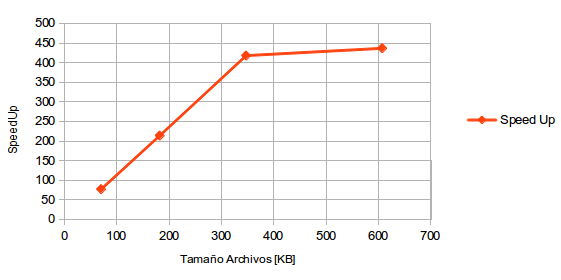
\includegraphics[width=0.88\textwidth]{images/SpeedUpBubblevsHeap.png}
		\medskip
		\caption{Gráfico del speedup del Bubblesort contra el Heapsort.}
	\end{figure}
	\bigskip\bigskip


	En el segundo caso, se compara el tiempo de ejecución del algoritmo \textit{Heapsort} en sus dos versiones: la que genera el compilador de C y la que fue diseñada e implementada en Assembly de MIPS32. Como se observa en la \textit{Figura 2}, el algoritmo con mejor performance fue el diseñado para Assembly de MIPS32. Se debe notar que al compilar con \textit{GCC} no se le agregó ninguna optimización al código de Assembly (opción por default al compilar). 
	\bigskip

	% Tabla 2
	\begin{table}[!hbt]
		\begin{center}
		\begin{tabular}{|>{\centering\arraybackslash}m{5cm}|>{\centering \arraybackslash}m{4cm}|>{\centering \arraybackslash}m{3cm}|}
			\hline
			\rowcolor[gray]{0.9}\textbf{Nombre de Archivo} & \textbf{Tiempo Heapsort MIPS32} & \textbf{Tiempo heapsort C}\\
			\hline
			\centering 25deMayo.txt & 3,395s & 3,883s \\
			\hline
			\centering argentina.txt & 13,367s & 15,469s \\
			\hline
			\centering cookbook.txt & 1,148s & 1,383s \\
			\hline
			\centering 2pac.txt & 6,715s & 7,371s \\
			\hline
		\end{tabular}
		\smallskip
		\caption{Tiempos obtenidos en la ejecución\\ del algoritmo Heapsort para distintos archivos de entrada.}
		\end{center}
	\end{table}
	\bigskip

	% Gráfico de barras de la performance
	\begin{figure}[H]
	\centering
	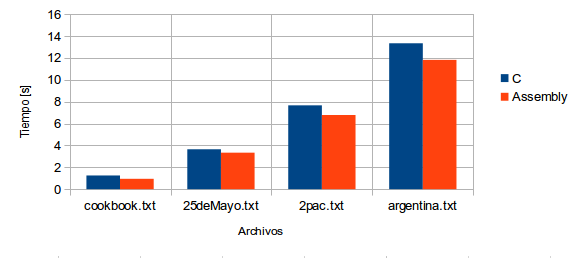
\includegraphics[width=0.88\textwidth]{images/CvsMips.png}
	\medskip
		\caption{Gráfico comparando la performance del Heapsort\\ en sus dos implementaciones (C vs Assembly).}
	\end{figure}
	\bigskip\bigskip\bigskip


	En la \textit{Figura 3} se observa el speedup del Heapsort en C contra la versión en Assembly.
	\bigskip


	% Grafico del speedup
	\begin{figure}[H]
		\centering
		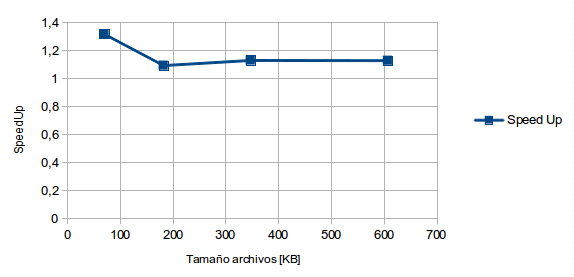
\includegraphics[width=0.88\textwidth]{images/SpeedUpCvsAssembly.png}
		\medskip
		\caption{Gráfico del speedup del Heapsort en C contra\\ la versión en Assembly.}
	\end{figure}
	\bigskip\bigskip


\section{Conclusiones}

	Se puede observar que existen diferencias significativas entre los algoritmos Bubblesort y el Heapsort, con respecto a los tiempos de ejecución. Es notable que el Bubblesort es inferior en cuanto a la performance comparado con el Heapsort (ambos implementados en C). Esto se puede corroborar observando el speedup obtenido.

	También se pueden ver las diferencias en el Heapsort en sus dos implementaciones: en C y em Assembly MIPS32. Los tiempos de ejecución de ambos son muy similares, pero se puede observar que la versión diseñada para Assembly es apenas mejor. También se puede corroborar esto observando el speedup obtenido.

\bigskip


% Citas bibliográficas.
\begin{thebibliography}{99}

	\bibitem{BS} Bubblesort, \url{http://en.wikipedia.org/wiki/Bubble_sort}

	\bibitem{HS} Heapsort, \url{http://en.wikipedia.org/wiki/Heapsort}

	\bibitem{GXEMUL} The NetBSD project, \url{http://www.netbsd.org/}

	\bibitem{GCC} GCC, the GNU Compiler Collection, \url{http://gcc.gnu.org/}

	\bibitem{TIME} time man page, \url{http://unixhelp.ed.ac.uk/CGI/man-cgi?time}

	\bibitem{ABI} MIPS ABI, \url{http://www.sco.com/developers/devspecs/mipsabi.pdf}

	\bibitem{HEN00} J. L. Hennessy and D. A. Patterson, ``Computer Architecture. A Quantitative
	Approach,'' 4th Edition, Morgan Kaufmann Publishers, 2000.

	\end{thebibliography}

\newpage


% Apendices
\begin{appendices}

\bigskip\bigskip

% Implementación completa en lenguaje C
\section{Implementación completa en lenguaje C}


\subsection{\textit{tp1.c}. Implementación del main del programa}
% Código
\lstset{ language = C } % Cambiamos el lenguaje para que parsee en C
\lstinputlisting[label=codeTP0cfull,caption=``tp1.c'']{../codigo/c/tp1.c} 
\bigskip\bigskip

\subsection{\textit{bubblesort.h}. Declaración del algoritmo Bubblesort}
% Código
\lstset{ language = C } % Cambiamos el lenguaje para que parsee en C
\lstinputlisting[label=codeBShfull,caption=``bubblesort.h'']{../codigo/c/bubblesort.h} 
\bigskip\bigskip

\subsection{\textit{bubblesort.c}. Definición del algoritmo Bubblesort}
% Código
\lstset{ language = C } % Cambiamos el lenguaje para que parsee en C
\lstinputlisting[label=codeBScfull,caption=``bubblesort.c'']{../codigo/c/bubblesort.c} 
\bigskip\bigskip

\subsection{\textit{heapsort.h}. Declaración del algoritmo Heapsort}
% Código
\lstset{ language = C } % Cambiamos el lenguaje para que parsee en C
\lstinputlisting[label=codeBShfull,caption=``heapsort.h'']{../codigo/c/heapsort.h} 
\bigskip\bigskip

\subsection{\textit{heapsort.c}. Definición del algoritmo Heapsort}
% Código
\lstset{ language = C } % Cambiamos el lenguaje para que parsee en C
\lstinputlisting[label=codeBScfull,caption=``heapsort.c'']{../codigo/c/heapsort.c} 
\newpage



% Implementación completa en lenguaje C
\section{Implementación completa en lenguaje Assembly MIPS32}


\subsection{\textit{tp1.c}. Implementación del main del programa}
% Código
\lstset{ language =C } % Cambiamos el lenguaje para que parsee en MIPS
\lstinputlisting[label=codeTP0cfull,caption=``tp1.c'']{../codigo/assembly/tp1.c} 
\bigskip\bigskip

\subsection{\textit{heapsort.S}. Definición del algoritmo Heapsort}
% Código
\lstset{ language = [mips]Assembler} % Cambiamos el lenguaje para que parsee en MIPS
\lstinputlisting[label=codeTP0cfull,caption=``heapsort.S'']{../codigo/assembly/heapsort.S} 
\bigskip\bigskip

\subsection{\textit{heap.S}. Definición del algoritmo Heap}
% Código
\lstset{ language = [mips]Assembler} % Cambiamos el lenguaje para que parsee en MIPS
\lstinputlisting[label=codeTP0cfull,caption=``heap.S'']{../codigo/assembly/heap.S} 
\bigskip\bigskip

\subsection{\textit{strcmpi.S}. Definición del algoritmo Strcmpi}
% Código
\lstset{ language = [mips]Assembler} % Cambiamos el lenguaje para que parsee en MIPS
\lstinputlisting[label=codeTP0cfull,caption=``strcmpi.S'']{../codigo/assembly/strcmpi.S} 
\bigskip\bigskip


\end{appendices}

\end{document}
